\documentclass[border=0.65cm,tikz]{standalone}
\usepackage[utf8]{vietnam}
\usepackage{xcolor}
\definecolor{dnvang}{HTML}{D8A25E}
\definecolor{dnxanh}{HTML}{229799}
\definecolor{dnxanhdam}{HTML}{0D7C66}
\definecolor{dndo}{HTML}{BB2649}
\def\mycolor{dnvang}
\def\mauphu{dnxanh}
\def\maudam{dnxanhdam}
\def\maunhan{dndo}
\usepackage{tikz}
\usepackage{tikz-3dplot}
\usepackage{pgfplots}
\pgfplotsset{compat=1.18}
\usetikzlibrary{angles,quotes,intersections,fit}
\usetikzlibrary{calc,fadings,shadows,shadows.blur,shapes,shapes.geometric,positioning,backgrounds,decorations.pathmorphing,decorations,matrix}
\usetikzlibrary{decorations.pathmorphing}
\begin{document}
%%%Sự hình thành liên kết H2
	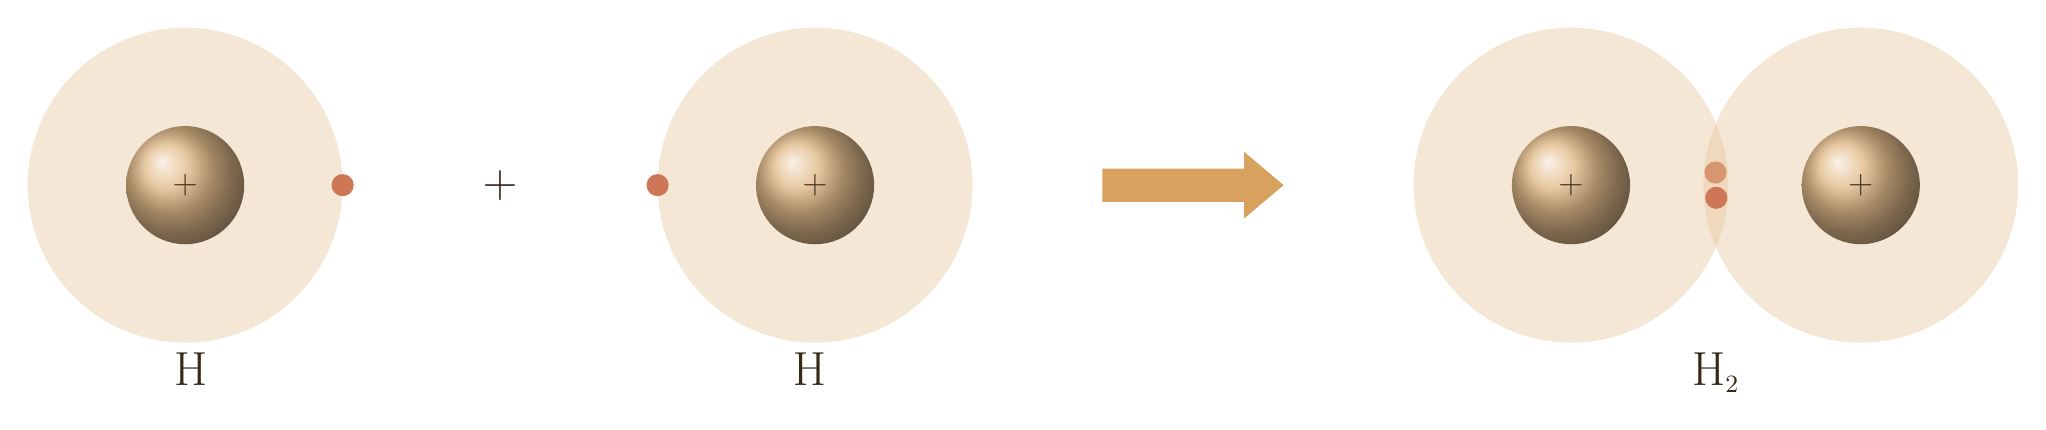
\begin{tikzpicture}[declare function={%
			r1=0.75cm;
			r2=2.0cm;
			d=8cm;
		}
		]%
		\tikzset{
			hirdrogen/.pic={
				\path[fill=\mycolor!65,opacity =0.4,pic actions] (0,0) circle (r2);
				\path[ball color=\mycolor!80,opacity =0.9,pic actions] (0,0) circle (r1) node[font=\large\fontfamily{qag}\selectfont,text=\mycolor!25!black] {$\textbf{+}$};
				\foreach \g/\r in{0/r2}{%
					\fill (\g:\r) [\maunhan!35!\mycolor] circle (4pt);
				}
				%%
			},
			hirdrogenH/.pic={
				\path[fill=\mycolor!65,opacity =0.4,pic actions] (0,0) circle (r2);
				\path[ball color=\mycolor!80,opacity =0.9,pic actions] (0,0) circle (r1) node[font=\large\fontfamily{qag}\selectfont,text=\mycolor!25!black] {$\textbf{+}$};
				\foreach \g/\r in{5/r2-4.5pt}{%
					\fill (\g:\r) [\maunhan!35!\mycolor] circle (4pt);
				}
				%%
			},
			stylefont/.style={font=\bfseries\LARGE\fontfamily{qag}\selectfont,text=\mycolor!25!black}
		}
		%%%Vẽ nguyen tử thứ nhất
		\path (0,0) pic[local bounding box =na] {hirdrogen};
		\path (na.south) node[anchor=north,stylefont] {H};
		%%%%vẽ dấu cộng
		\path (0.5*d,0) node[stylefont] {+};
		%%%Vẽ nguyen tử thứ hai
		\path (d,0) pic[rotate=180, local bounding box =nb] {hirdrogen};
		\path (nb.south) node[anchor=north,stylefont] {H};
		\path (1.6*d,0) node {
			\tikz{
				\fill[\mycolor](0,0)--++(-90:6pt) coordinate (A)
				--++(-1.8cm,0)--++(-90:12pt)--++(0:1.8cm)coordinate (B)
				--++(-90:6pt)--($(A)!0.5!(B)+(0.5cm,0)$)--cycle;
			}
		};
		%%%Vẽ phân tử hirdrogen
		\path (2.2*d,0) pic[local bounding box =nc] {hirdrogenH};
		\path (2.66*d,0) pic[rotate=180,local bounding box =nd] {hirdrogenH};
		\path ($(nc.south)!0.5!(nd.south)$) node [anchor=north,stylefont] {H$_\textbf{\small2}$};
	\end{tikzpicture}
\end{document}